\begin{equation}
    \begin{gathered}
        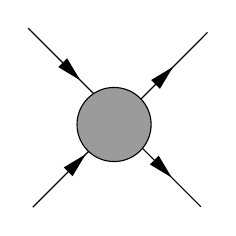
\begin{tikzpicture}[x=0.75pt,y=0.75pt,yscale=-1,xscale=1]
            %uncomment if require: \path (0,300); %set diagram left start at 0, and has height of 300
            
            %Straight Lines [id:da9345131028574916] 
            \draw    (152.5,157.2) -- (202.71,207.41) ;
            \draw [shift={(177.6,182.3)}, rotate = 225] [fill={rgb, 255:red, 0; green, 0; blue, 0 }  ][line width=0.08]  [draw opacity=0] (12,-3) -- (0,0) -- (12,3) -- cycle    ;
            %Straight Lines [id:da39542753625606863] 
            \draw    (207.71,215.2) -- (235.71,243.2) ;
            \draw [shift={(221.71,229.2)}, rotate = 225] [fill={rgb, 255:red, 0; green, 0; blue, 0 }  ][line width=0.08]  [draw opacity=0] (12,-3) -- (0,0) -- (12,3) -- cycle    ;
            %Straight Lines [id:da2774188281079233] 
            \draw    (154.71,243.41) -- (205.71,192.41) ;
            \draw [shift={(180.21,217.91)}, rotate = 495] [fill={rgb, 255:red, 0; green, 0; blue, 0 }  ][line width=0.08]  [draw opacity=0] (12,-3) -- (0,0) -- (12,3) -- cycle    ;
            %Straight Lines [id:da36864179204173797] 
            \draw    (205.71,192.41) -- (238.91,159.2) ;
            \draw [shift={(222.31,175.8)}, rotate = 495] [fill={rgb, 255:red, 0; green, 0; blue, 0 }  ][line width=0.08]  [draw opacity=0] (12,-3) -- (0,0) -- (12,3) -- cycle    ;
            %Shape: Circle [id:dp41808205207920834] 
            \draw  [fill={rgb, 255:red, 155; green, 155; blue, 155 }  ,fill opacity=1 ] (176,203.59) .. controls (176,193.73) and (183.99,185.73) .. (193.85,185.73) .. controls (203.71,185.73) and (211.71,193.73) .. (211.71,203.59) .. controls (211.71,213.45) and (203.71,221.44) .. (193.85,221.44) .. controls (183.99,221.44) and (176,213.45) .. (176,203.59) -- cycle ;
            \end{tikzpicture}                
    \end{gathered} = \begin{gathered}
        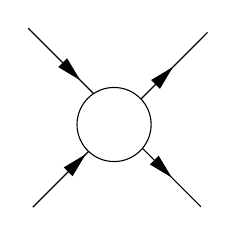
\begin{tikzpicture}[x=0.75pt,y=0.75pt,yscale=-1,xscale=1]
            %uncomment if require: \path (0,300); %set diagram left start at 0, and has height of 300
            
            %Straight Lines [id:da9345131028574916] 
            \draw    (152.5,157.2) -- (202.71,207.41) ;
            \draw [shift={(177.6,182.3)}, rotate = 225] [fill={rgb, 255:red, 0; green, 0; blue, 0 }  ][line width=0.08]  [draw opacity=0] (12,-3) -- (0,0) -- (12,3) -- cycle    ;
            %Straight Lines [id:da39542753625606863] 
            \draw    (207.71,215.2) -- (235.71,243.2) ;
            \draw [shift={(221.71,229.2)}, rotate = 225] [fill={rgb, 255:red, 0; green, 0; blue, 0 }  ][line width=0.08]  [draw opacity=0] (12,-3) -- (0,0) -- (12,3) -- cycle    ;
            %Straight Lines [id:da2774188281079233] 
            \draw    (154.71,243.41) -- (205.71,192.41) ;
            \draw [shift={(180.21,217.91)}, rotate = 495] [fill={rgb, 255:red, 0; green, 0; blue, 0 }  ][line width=0.08]  [draw opacity=0] (12,-3) -- (0,0) -- (12,3) -- cycle    ;
            %Straight Lines [id:da36864179204173797] 
            \draw    (205.71,192.41) -- (238.91,159.2) ;
            \draw [shift={(222.31,175.8)}, rotate = 495] [fill={rgb, 255:red, 0; green, 0; blue, 0 }  ][line width=0.08]  [draw opacity=0] (12,-3) -- (0,0) -- (12,3) -- cycle    ;
            %Shape: Circle [id:dp41808205207920834] 
            \draw  [fill={rgb, 255:red, 255; green, 255; blue, 255 }  ,fill opacity=1 ] (176,203.59) .. controls (176,193.73) and (183.99,185.73) .. (193.85,185.73) .. controls (203.71,185.73) and (211.71,193.73) .. (211.71,203.59) .. controls (211.71,213.45) and (203.71,221.44) .. (193.85,221.44) .. controls (183.99,221.44) and (176,213.45) .. (176,203.59) -- cycle ;
            \end{tikzpicture}                    
    \end{gathered} + \begin{gathered}
        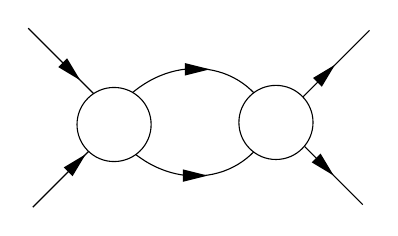
\begin{tikzpicture}[x=0.75pt,y=0.75pt,yscale=-1,xscale=1]
            %uncomment if require: \path (0,300); %set diagram left start at 0, and has height of 300
            
            %Curve Lines [id:da0323321140047681] 
            \draw    (165.71,161.41) .. controls (188.71,190.79) and (225.71,187.79) .. (239.71,161.79) ;
            %Straight Lines [id:da23429070529223384] 
            \draw    (211,182.2) ;
            \draw [shift={(211,182.2)}, rotate = 180] [fill={rgb, 255:red, 0; green, 0; blue, 0 }  ][line width=0.08]  [draw opacity=0] (12,-3) -- (0,0) -- (12,3) -- cycle    ;
            %Curve Lines [id:da006405555941071395] 
            \draw    (165.71,151.59) .. controls (188.71,122.21) and (225.71,125.21) .. (239.71,151.21) ;
            %Straight Lines [id:da7859806184703646] 
            \draw    (124.5,111.2) -- (174.71,161.41) ;
            \draw [shift={(149.6,136.3)}, rotate = 225] [fill={rgb, 255:red, 0; green, 0; blue, 0 }  ][line width=0.08]  [draw opacity=0] (12,-3) -- (0,0) -- (12,3) -- cycle    ;
            %Straight Lines [id:da979040764755357] 
            \draw    (126.71,197.41) -- (177.71,146.41) ;
            \draw [shift={(152.21,171.91)}, rotate = 495] [fill={rgb, 255:red, 0; green, 0; blue, 0 }  ][line width=0.08]  [draw opacity=0] (12,-3) -- (0,0) -- (12,3) -- cycle    ;
            %Shape: Circle [id:dp6186819574350089] 
            \draw  [fill={rgb, 255:red, 255; green, 255; blue, 255 }  ,fill opacity=1 ] (148,157.59) .. controls (148,147.73) and (155.99,139.73) .. (165.85,139.73) .. controls (175.71,139.73) and (183.71,147.73) .. (183.71,157.59) .. controls (183.71,167.45) and (175.71,175.44) .. (165.85,175.44) .. controls (155.99,175.44) and (148,167.45) .. (148,157.59) -- cycle ;
            %Straight Lines [id:da26833664483472486] 
            \draw    (257.71,168.2) -- (285.71,196.2) ;
            \draw [shift={(271.71,182.2)}, rotate = 225] [fill={rgb, 255:red, 0; green, 0; blue, 0 }  ][line width=0.08]  [draw opacity=0] (12,-3) -- (0,0) -- (12,3) -- cycle    ;
            %Straight Lines [id:da4482068470519842] 
            \draw    (255.71,145.41) -- (288.91,112.2) ;
            \draw [shift={(272.31,128.8)}, rotate = 495] [fill={rgb, 255:red, 0; green, 0; blue, 0 }  ][line width=0.08]  [draw opacity=0] (12,-3) -- (0,0) -- (12,3) -- cycle    ;
            %Shape: Circle [id:dp8625776854304812] 
            \draw  [fill={rgb, 255:red, 255; green, 255; blue, 255 }  ,fill opacity=1 ] (226,156.59) .. controls (226,146.73) and (233.99,138.73) .. (243.85,138.73) .. controls (253.71,138.73) and (261.71,146.73) .. (261.71,156.59) .. controls (261.71,166.45) and (253.71,174.44) .. (243.85,174.44) .. controls (233.99,174.44) and (226,166.45) .. (226,156.59) -- cycle ;
            %Straight Lines [id:da5905789317550543] 
            \draw    (212,131) ;
            \draw [shift={(212,131)}, rotate = 180] [fill={rgb, 255:red, 0; green, 0; blue, 0 }  ][line width=0.08]  [draw opacity=0] (12,-3) -- (0,0) -- (12,3) -- cycle    ;
            \end{tikzpicture}            
    \end{gathered} + \cdots,
\end{equation}